\documentclass[tikz,border=7pt]{standalone}
\usepackage{amsmath,amssymb}
\usetikzlibrary{arrows.meta,patterns,decorations.markings,calc}
\tikzset{outline/.style={line width=.7pt,line cap=round,line join=round},
 map/.style={outline,-{Stealth[length=2.1mm,width=1.5mm]}},
 point/.style={circle,draw,fill=white,inner sep=1.4pt,line width=.6pt},
 along/.style={postaction={decorate},decoration={markings,mark=at position .52 with {\arrow{Stealth[length=1.8mm,width=1.2mm]}}}}}
\begin{document}
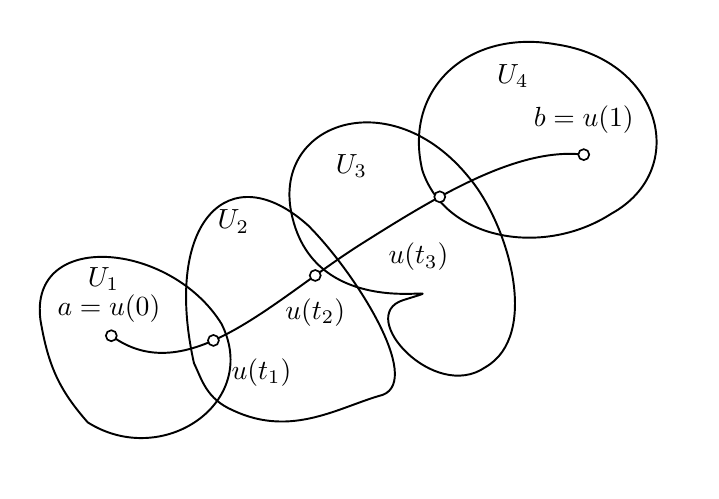
\begin{tikzpicture}[font=\normalsize]

\draw[outline] (-.75,.4) .. controls (-.9,1.55) and (.9,1.4) .. (1.55,.35) .. controls (2.05,-.65) and (.8,-1.5) .. (-.15,-.9) .. controls (-.5,-.5) and (-.65,-.2) .. (-.75,.4) -- cycle;
\draw[outline] (1.2,-.15) .. controls (.8,1.65) and (1.65,2.5) .. (2.65,1.6) .. controls (3.25,1) and (4.1,-.35) .. (3.6,-.55) .. controls (3.05,-.7) and (2.45,-1.1) .. (1.7,-.75) .. controls (1.35,-.6) and (1.3,-.35) .. (1.2,-.15) -- cycle;
\draw[outline] (2.45,1.7) .. controls (2.15,2.9) and (3.7,3.45) .. (4.7,2.2) .. controls (5.2,1.6) and (5.6,.2) .. (4.9,-.2) .. controls (4.25,-.65) and (3.25,.45) .. (3.85,.65) .. controls (4.8,.95) and (2.8,.25) .. (2.45,1.7) -- cycle;
\draw[outline] (4.1,2.3) .. controls (3.85,3.35) and (4.7,4.1) .. (5.8,3.9) .. controls (7.15,3.7) and (7.5,2.3) .. (6.5,1.75) .. controls (5.65,1.2) and (4.4,1.4) .. (4.1,2.3) -- cycle;
\draw[outline] (.15,.2) .. controls (1.1,-.5) and (2.2,.65) .. (3.3,1.35) coordinate[pos=.43] (t1) coordinate[pos=.83] (t2) .. controls (4.25,1.95) and (5.3,2.6) .. (6.15,2.5) coordinate[pos=.35] (t3);
\node[point] at (.15,.2) {};\node at (.12,.55) {$a=u(0)$};
\node[point] at (6.15,2.5) {};\node[above=4pt] at (6.15,2.5) {$b=u(1)$};
\node at (.05,.92) {$U_1$};\node at (1.7,1.65) {$U_2$};\node at (3.2,2.35) {$U_3$};\node at (5.25,3.5) {$U_4$};
\node[point] at (t1) {};\node[below right=3pt] at (t1) {$u(t_1)$};
\node[point] at (t2) {};\node[below=5pt] at (t2) {$u(t_2)$};
\node[point] at (t3) {};\node at (4.05,1.2) {$u(t_3)$};

\end{tikzpicture}
\end{document}
